\documentclass[12pt]{article}
\usepackage{graphicx} % Required for inserting images
\usepackage[T2A]{fontenc}
\usepackage{geometry} % Managing page fields
\geometry{top=2cm, bottom=2cm, left=3cm, right=2cm}
\usepackage{booktabs}

\title{Дизайн документ}
\author{Авербух Семён, Бычкова Антонина, \\ Карташов Никита, Монёв Кирилл}
\date{Ноябрь 2024}

\sloppy
\begin{document}

\maketitle

% Уменьшаем шрифт только для оглавления
\begingroup
\footnotesize
\tableofcontents
\endgroup

\section{Введение}
Данный дизайн-документ знакомит с концепцией и спецификацией разрабатывающейся игры. Целью документа является создание структурированного и подробного описания множества аспектов игры, начиная от самой концепции и заканчивая техническими деталями реализации.

Игра разрабатывается как 2D-проект с видом сверху, где сюжет и сражения являются основным акцентом. Вдохновением для игры послужили такие проекты, как \textit{Hotline Miami} и \textit{Dead Cells}.

Цель игры — познакомить игрока с историей о борьбе и внутреннем росте главного героя, дать возможность поучаствовать в увлекательных сражениях и самому выбирать, как будут развиваться события. Игрок получит уникальный опыт взаимодействия с динамичным игровым миром, а также сможет проверить свои интеллектуальные способности.

\section{Концепция}
    \subsection{Введение}
Игра переносит игрока в суровую, но одновременно уютную реальность российской глубинки, начинающийся с мрачной атмосферы квартиры главного героя. Одновременно с тем, как игрок проходит испытания и раскрывает сюжет, обстановка вокруг становится светлее, передавая внутреннюю трансформацию персонажа.

Основная идея игры — показать, что даже в самых трудных условиях можно найти путь к улучшению и изменению себя и своего мира.
    \subsection{Жанр и аудитория}
    \textbf{Жанр:} 2D экшн с сюжетом и элементами головоломки.
    \subsection{Основные особенности игры}
    \begin{enumerate}
    \item \textbf{Вид сверху и 2D-графика} — обеспечивает простой и понятный геймплей.
    \item \textbf{Развитие сюжета} — история героя является центральной частью игры.
    \item \textbf{Смена атмосферы} — визуальный стиль отражает прогресс игрока, от серых и мрачных тонов к более ярким и насыщенным.
    \item \textbf{Разнообразие сражений} — использование холодного и огнестрельного оружия.
    \item \textbf{Интерактивность} — возможность взаимодействовать с предметами, решать головоломки.
\end{enumerate}
    \subsection{Описание игры}
    Главный герой — обычный парень, вынужденный противостоять алкашам, гопникам, тараканам и прочим персонажам, встречающимся на пути. Игрок перемещается по комнатам, участвуя в сражениях и исследуя окружающий мир. Игра представляет собой череду комнат и локаций, каждая из которых предлагает новые испытания.

    В начале игрок сталкивается с унылой обстановкой, но по мере прохождения и развития сюжета мир вокруг него меняется. Герой становится сильнее, открывает новые возможности и навыки. Атмосфера игры постепенно трансформируется, отражая внутреннюю эволюцию героя: от мрачных и приглушённых тонов — к насыщенным и жизнеутверждающим, что символизирует его рост и способность справляться с трудностями.
    \subsection{Предпосылки создания}
    \setlength{\parindent}{1.5em}В последние годы наблюдается заметный рост интереса к 2D-играм, особенно среди инди-разработчиков. Игры с пиксельной графикой и уникальным художественным стилем привлекают внимание как новых, так и опытных игроков. Успех таких проектов, как Celeste, Hollow Knight и Katana ZERO, подтверждает, что аудитория готова поддерживать качественные 2D-игры, предлагающие интересный геймплей и захватывающую атмосферу. Помимо этого, современные игроки все чаще ищут уникальные комбинации жанров. Hotline Miami и Dead Cells представляют собой разные подходы к экшену, и их сочетание может создать новый, увлекательный опыт. Игры, которые успешно смешивают элементы различных жанров, часто становятся популярными, так как они предлагают игрокам разнообразие и новизну.
    
        \setlength{\parindent}{1.5em}Важно отметить, что создание игры, вдохновленной Hotline Miami и Dead Cells, не подразумевает прямого копирования их контента. Лицензирование и авторские права защищают конкретные механики, персонажей и сюжетные линии, но не идеи и концепции.
    \subsection{Платформа}
    Создание игры планируется на PC(Windows). Ниже перечислены минимальные и рекомендованные системные требования.
    \begin{table}[h]
    \centering
    \begin{tabular}{|l|l|l|} % Добавлены вертикальные линии
        \hline
        \textbf{Требования} & \textbf{Минимальные} & \textbf{Рекомендуемые} \\ 
        \hline
        Операционная система & Windows 7 & Windows 10 \\ 
        \hline
        Процессор & 2.0 GHz Dual-Core & 3.0 GHz Quad-Core \\ 
        \hline
        Оперативная память (ОЗУ) & 4 GB RAM & 8 GB RAM \\ 
        \hline
        Видеокарта & NVIDIA GeForce 660 & NVIDIA GeForce GTX 970 \\ 
        \hline
        Место на диске & 2 GB & 4 GB \\ 
        \hline
        Свободное место на HDD & 2 GB & 4 GB \\ 
        \hline
        CD-ROM привод & Не требуется & Не требуется \\ 
        \hline
        Звуковая карта & Совместимая с DirectX & Совместимая с DirectX \\ 
        \hline
        Управление & Клавиатура и мышь & Клавиатура и мышь / Gamepad \\ 
        \hline
    \end{tabular}
    \end{table}


\section{Функциональная спецификация}
    \subsection{Принципы игры}
        \subsubsection{Суть игрового процесса}
        Игровой процесс в игре строится вокруг динамичных сражений и взаимодействия с окружающим миром. Игрок управляет главным героем, который постепенно становится сильнее, открывает новые возможности и проходит через испытания, преодолевая врагов и раскрывая сюжет.  
    
        Основное развлечение для игрока заключается в сочетании тактического выбора и быстрых, захватывающих схваток. Благодаря разнообразию врагов и уникальному подходу к сражениям, игроку придется адаптироваться к разным ситуациям, использовать холодное и огнестрельное оружие, а также наиболее эффективно взаимодействовать окружением.  
    
        В основе игрового процесса лежит идея, что каждый бой – это серьезное испытание. Игроку нужно учитывать слабости врагов, особенности своего оружия, а также расположение объектов на карте. Например, взрывоопасные бочки, укрытия или тесные проходы могут играть ключевую роль в сражении. Это добавляет глубину и заставляет игрока экспериментировать, подстраивая свою стратегию под новые условия.  
    
        Игра стремится создать опыт, который объединяет напряженность и удовольствие от победы. Каждый бой – это маленький вызов, который будет держать игрока в напряжении и позволять ему почувствовать себя настоящим героем, преодолевающим трудности.  
    
        Интерфейс будет интуитивно понятным, а управление – отзывчивым, чтобы максимально облегчить процесс вовлечения. Цель игры – подарить игроку эмоции: от чувства упадка в начале, до эйфории побед и прогресса в конце.  
    
        \subsubsection{Ход игры и сюжет}
        Игровой процесс делится на эпизоды, каждый из которых представляет собой набор комнат, связанных между собой. Каждая комната – это либо бой, либо интерактивная сцена, в которой можно собрать предметы, поговорить с NPC, или выполнить небольшой квест.  
    
        Типичный игровой сеанс начинается с того, что игрок оказывается в комнате, где его ждет какое-либо задание. Враги, такие как гопники, алкаши и даже тараканы, будут расставлены так, чтобы создавать вызовы. Игрок должен решить, каким оружием воспользоваться и как лучше всего подойти к ситуации.  
    
        На протяжении игры главный герой будет сталкиваться с новыми типами врагов, которые становятся умнее и опаснее. Каждый новый этап игры представляет усложнение: меняются как механики сражений, так и дизайн уровней. Например, узкие коридоры сменяются просторными помещениями, добавляются ловушки, а иногда герою придется использовать не только силу, но и смекалку.  
    
        Сюжет начинается с мрачной квартиры героя, где все буквально пропитано тоской и безысходностью. Первые враги – это тараканы и типичные бытовые раздражители, символизирующие внутреннюю апатию героя. 
    
        В процессе игрок узнает больше о прошлом героя, его мотивах и внутреннем состоянии. По мере продвижения обстановка меняется: унылые серые тона постепенно уступают место ярким краскам, окружающая среда становится все более красочной. Финальные эпизоды игры должны создать у игрока ощущение завершения пути: как будто он помог герою найти себя и изменить мир вокруг.  
    
        Каждая игровая сессия приносит не только прогресс, но и чувство достижения. Ключевая идея – показать, что путь преодоления трудностей, хотя и сложен, приносит внутреннюю награду. Это не только экшен, но и эмоциональная история, в которой игрок почувствует, что его действия имеют значение.  
    
        В игре будет много мелких деталей, которые оживляют мир: например, записки, оставленные на стенах, дневники NPC или небольшие шутки, спрятанные в диалогах. Все это должно создать ощущение, что мир игры живой, а история глубока и многослойна.
    \subsection{Физическая модель}

        Физическая модель игры создаёт интуитивно понятный и динамичный игровой процесс. Игра сосредоточена на простоте и удобстве взаимодействия с окружением, чтобы игрок мог наслаждаться сражениями и исследованием, не отвлекаясь на сложные физические механики.
        
        \subsubsection{Перемещения}
        
        \begin{itemize}
            \item \textbf{Движение персонажа:} Главный герой может свободно перемещаться в любом направлении по локации с фиксированной скоростью. Его движения плавные, с мгновенной реакцией на команды игрока.
            \begin{itemize}
                \item \textbf{W} — движение вверх.
                \item \textbf{A} — движение влево.
                \item \textbf{S} — движение вниз.
                \item \textbf{D} — движение вправо.
            \end{itemize}
            \item \textbf{Препятствия:} Столкновения с предметами, такими как стены или мебель, приводят к остановке движения. Маленькие предметы, например, бутылки, могут быть сдвинуты или перевёрнуты.
        \end{itemize}
        
        \subsubsection{Боевые действия}
        
        \begin{itemize}
            \item \textbf{Холодное оружие:} Удары совершаются мгновенно, анимации короткие. Разные виды оружия отличаются скоростью атаки и нанесённым уроном. Например, нож быстрый, но менее мощный, а лом медленный, но разрушительный.
            \item \textbf{Огнестрельное оружие:} Стрельба осуществляется мгновенно, пули попадают точно в цель. Боеприпасы ограничены.  Это создает необходимость для игрока использовать их с умом, подстраивая свои действия под доступные патроны. Игрок может искать дополнительные боеприпасы в различных локациях, что добавляет элемент исследования и стимулирует стратегический подход к каждому сражению.
            \begin{itemize}
                \item \textbf{Пистолеты:} 
                \begin{itemize}
                    \item Идеальны для быстрых выстрелов и мобильности.
                    \item Меньшая мощность по сравнению с другими видами оружия.
                    \item Высокая скорость перезарядки.
                \end{itemize}
                \item \textbf{Дробовики:} 
                \begin{itemize}
                    \item Мощные на близких расстояниях.
                    \item Ограниченная дальнобойность.
                    \item Низкая скорострельность.
                \end{itemize}
                \item \textbf{Автоматы:} 
                \begin{itemize}
                    \item Высокая скорострельность.
                    \item Быстрое расходование патронов.
                    \item Хороши для массовых сражений на средних и близких расстояниях.
                \end{itemize}
            \end{itemize}
            \item \textbf{Враги:} 
                \begin{itemize}
                    \item При попадании враги могут быть сбиты с ног или отлететь, в зависимости от силы удара и используемого оружия.
                    \item Враги могут иметь разное количество здоровья, что влияет на их поведение в бою. Например, одни враги могут погибать от одного удара, а другие — требовать несколько попаданий.
                    \item Враги могут атаковать как в ближнем бою (с использованием оружия или без него), так и на расстоянии, используя огнестрельное оружие.
                    \item Некоторые враги могут использовать укрытия, чтобы избегать попаданий, или пытаться окружить игрока, что заставляет его быть более внимательным и постоянно двигаться.
                    \item Некоторые типы врагов обладают особыми атаками, например, могут бросать взрывчатку или устанавливать ловушки, что добавляет элемент неожиданности и стратегической сложности.
                \end{itemize}
        \end{itemize}
        
        \subsubsection{Взаимодействие с окружением}

            \begin{itemize}
                \item \textbf{Использование укрытий:} 
                \begin{itemize}
                    \item Игрок может прятаться за различными объектами на уровне, такими как мебель, стены, ящики и другие препятствия. Укрытия позволяют избегать огня врагов, защищать себя от выстрелов и подстраивать тактику нападения.
                    \item Некоторые укрытия могут быть разрушимыми, что добавляет динамичности в бою. Игрок должен учитывать, насколько долго он может оставаться за укрытием, прежде чем оно разрушится или будет уничтожено врагами.
                \end{itemize}
                
                \item \textbf{Ловушки:} 
                    Некоторые уровни могут включать в себя ловушки, такие как острые шипы или электрические проводки, которые будут наносить урон игроку.
                \item \textbf{Взаимодействие с окружающими элементами:}
                        На уровнях будут встречаться ящики, в которых можно приобрести оружие за собранные монеты. Монеты можно найти, исследуя уровни, что мотивирует игрока к более детальному изучению карты.
            \end{itemize}

        
        \subsubsection{Общая атмосфера физики}
        
        Физика мира не усложняет игровой процесс, но дополняет его. Игрок всегда чувствует контроль над героем и его взаимодействиями, что создаёт погружение в атмосферу игры. Разрушения, звуки и эффекты делают каждое столкновение или действие запоминающимся.

    \subsection{Персонаж игрока}
        Главный герой представляет собой обычного молодого человека, живущего в серой и унылой реальности. Его внешний вид минималистичен: повседневная одежда (толстовка, футболка, джинсы) приглушённых оттенков, что подчёркивает его типичность и отсутствие ярко выраженной индивидуальности на начальных этапах.Его цель: Выйти из состояния апатии, преодолеть возникающие трудности и добиться личного роста, изменив мир вокруг себя.
    \subsection{Элементы игры}
    \subsubsection{Главный герой}
Главный герой — обычный парень, который начинает свое путешествие в мрачной квартире. Он может быть представлен в нейтральной цветовой гамме (чёрный, серый, белый), что подчеркивает его обыденность. По мере прохождения игры его внешний вид может изменяться в зависимости от выбора игрока и его успехов (например, новая одежда, аксессуары).

\subsubsection{Оружие}
Оружие в игре двух типов: холодное и огнестрельное.

\begin{itemize}
    \item \textbf{Холодное оружие:}
    \begin{itemize}
        \item \textbf{Нож.} Легкий и быстрый, позволяет совершать быстрые атаки. Имеет ограниченный радиус действия.
        \item \textbf{Лом.} Более мощное, но медленное оружие. Наносит большой урон, но требует времени на замах.
    \end{itemize}
    \item \textbf{Огнестрельное оружие:}
    \begin{itemize}
        \item \textbf{Пистолет.} Имеет ограниченный запас патронов, но позволяет наносить урон на расстоянии. Эффективен против более сильных врагов.
        \item \textbf{Дробовик.} Наносит большой урон на близком расстоянии, но имеет ограниченный радиус действия.
    \end{itemize}
\end{itemize}

\subsubsection{NPC}
В качестве NPC в игре присутствуют соседи по квартире, бармены и продавцы. В начальной локации игрок может встретить соседей, которые могут помочь. Они могут давать подсказки, предлагать квесты или просто комментировать происходящее. Бармены никак не взаимодействуют с игроком, ничего не говорят и не дают. В определенных локациях (на всех, кроме начальной) игрок сможет встретить торговцев, которые предлагают оружие, аптечки и другие предметы. Они будут выделяться внешне в отличие от других NPC.

\subsubsection{Локации}
В игре 3 локации:

\begin{itemize}
    \item \textbf{Квартира.} Начальная локация, темная и запущенная. Преобладают серые тона. Есть предметы мебели, техника, соседи, враги. Здесь игрок будет знакомиться с механиками игры и основами боя с несложными врагами.
    \item \textbf{Улица.} Пространство, где игрок может встретить более сильных врагов, чем в квартире. Здесь также будут находиться деревья, кусты, гаражи, дороги, мусорные баки, биотуалеты и продавцы.
    \item \textbf{Клуб.} Локация с наибольшим количеством предметов и врагов. Враги наиболее сильные. Преобладают яркие цвета: фиолетовый, желтый, красный, розовый. Среди предметов можно увидеть бар, джакузи, столы и стулья, сцену, танцпол, банкоматы, игровые автоматы и бильярдные столы.
\end{itemize}

\subsubsection{Взаимодействие с предметами}
Главный герой в процессе игры имеет возможность взаимодействовать с некоторыми предметами:

\begin{itemize}
    \item \textbf{Ящики.} Их можно открывать для поиска ресурсов и ключей.
    \item \textbf{Двери.} Игрок сможет открывать двери, что добавит элемент стратегии в игру.
    \item \textbf{Аптечки.} Позволяют восстанавливать здоровье. Их можно найти в разных местах, и они будут иметь разные уровни восстановления.
    \item \textbf{Компьютеры.} Необходимы для прохождения некоторых дополнительных квестов.
    \item \textbf{Ключи.} Необходимы для открытия дверей.
\end{itemize}

\subsubsection{Квесты и головоломки}
При прохождении всех представленных ниже квестов и головоломок будет вестись временной отсчёт, который будет использован для аналитики поведения игрока.

\begin{itemize}
    \item \textbf{"Пропавший ключ"} Главный герой обнаруживает, что дверь в следующую комнату заперта, а ключ пропал. Игроку нужно найти ключ, который был у одного из NPC, но тот не хочет его отдавать. Главный герой должен поговорить с NPC, чтобы узнать, где может находиться ключ. Каждый сосед будет давать подсказки о местонахождении ключа. Ключ может быть скрыт в одном из ящиков, которые игрок должен будет открыть, решив простую головоломку (например, комбинация из трех предметов, которые нужно расположить в правильном порядке) или правильно ответив на вопрос, связанный с самой игрой.
    \item \textbf{"Проблемы с соседями"} Игроку нужно помочь соседям решить их проблемы, чтобы они стали более дружелюбными и предоставили полезные ресурсы. Каждый сосед имеет свою уникальную проблему (например, потеря домашнего животного, проблемы с алкоголем, ссоры с другими соседями). Игрок должен будет выполнять квесты для каждого соседа, что может включать в себя поиск предметов, переговоры с другими NPC или сражения с врагами. После выполнения всех квестов соседи станут более дружелюбными и могут предложить игроку уникальные предметы или информацию, которые помогут в дальнейшем прохождении игры.
\end{itemize}


    \subsection{«Искусственный интеллект»}
            Искусственный интелект будет присущ различным противникам, в зависимости от их способностей и количества текущего здоровья, они будут по разному вести бой, убегать, взаимодействовать с предметами. Когда игрок вне поля зрения противника, то враги патрулируют местность или действуют согласно их роли и образа. Гопники: ходят в толпой или группой в несколько человек, бьют в среднем темпе и средней силой, отступают, если их остаётся мало или имеют мало хп. Омон: ходят в группе из нескольких человек, имеют слабые и быстрые атаки дубинками, дерутся до конца, держатся вместе при отступлении при малом кол-ве хп. Алкаши: ходят по одному или маленькими группами, имеют медлненную скорость ходьбы и атаки, имеют сильный,но неклюжий удар, не отступает даже при низком хп. 
    \subsection{Многопользовательский режим}
    \subsection{Интерфейс пользователя}
        \subsubsection{Блок-схема(картинка есть в репозитории)}
\begin{figure}
    \centering
    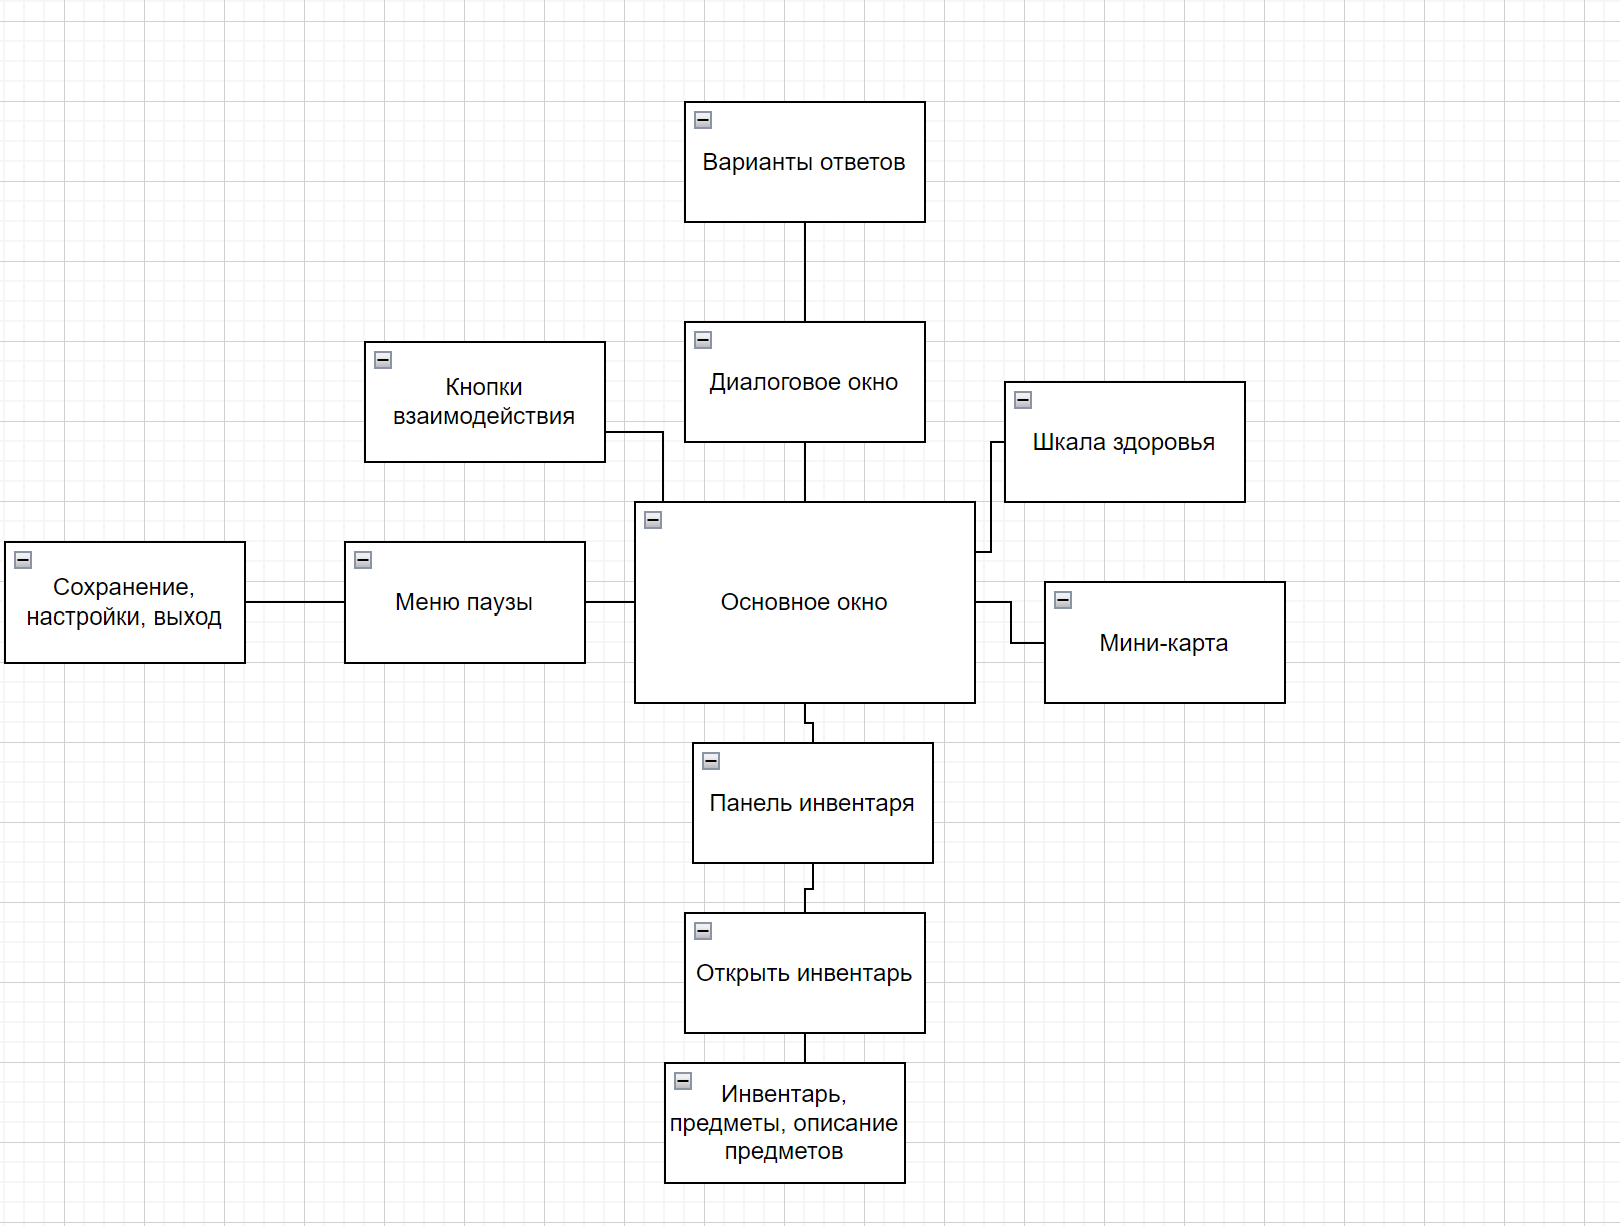
\includegraphics[width=0.5\linewidth]{image.png}
    \caption{Блок-схема игры}
    \label{fig:enter-label}
\end{figure}
        \subsubsection{Функциональное описание и управление}
        Этот раздел посвящен описанию функциональности интерфейса, логике работы каждого экрана и влиянию пользовательских действий на игровой процесс. Игра разработана для игры на ПК, что позволяет оптимизировать управление и взаимодействие через клавиатуру и мышь.  
        
        Интерфейс состоит из нескольких ключевых экранов:  
        \begin{itemize}
            \item \textbf{Главное меню.} Пользователь может начать игру или продолжить её, настроить параметры игры (управление, громкость), ознакомиться с инструкцией и выйти из игры.  
            \item \textbf{Экран игры.} Основной экран, на котором отображаются игровые элементы: состояние персонажа (здоровье), активное оружие, текущие задачи и игровой мир.  
            \item \textbf{Экран паузы.} Позволяет приостановить игру, настроить параметры, просмотреть текущее задание или выйти в главное меню.  
            \item \textbf{Экран завершения уровня.} Появляется после успешного выполнения задачи. Здесь отображается статистика: количество набранных очков, потраченное время, прогресс и возможность перейти к следующему уровню.  
        \end{itemize}
        
        Управление реализовано через сочетание клавиатуры и мыши: 
        \begin{itemize}
            \item \textbf{Клавиши управления движением.} WASD для передвижения, пробел для прыжка(переката), Shift для ускорения.  
            \item \textbf{Мышь.} Используется для прицеливания, атак и взаимодействия с элементами мира (например, открытие дверей или поднятие предметов).  
            \item \textbf{Клавиши быстрого доступа.} Например, 1-3 для смены оружия, E для взаимодействия с персонажами или диалоговыми окнами.  
        \end{itemize}
        
        Действия пользователя напрямую влияют на игровой процесс. Например, выбор оружия изменяет боевые тактики, а взаимодействие с игровыми объектами открывает доступ к новым зонам или ресурсам.
        
        \subsubsection{Объекты интерфейса пользователя}
        Интерфейс построен из стандартных и уникальных элементов, которые совместно создают интуитивное и удобное взаимодействие.
        
        \paragraph{Стандартные элементы}
        \begin{itemize}
            \item \textbf{Кнопки.} Используются в меню для навигации и подтверждения выбора. Например, кнопки «Начать игру», «Настройки», «Выход».  
            \item \textbf{Индикаторы.} Полоса здоровья героя размещена в верхнем левом углу, обеспечивая игроку информацию в любой момент.  
            \item \textbf{Текстовые уведомления.} Например, описание задания или напоминание о действиях («Нажмите E, чтобы открыть дверь»).  
        \end{itemize}
        
        \paragraph{Уникальные элементы}
        \begin{itemize}
            \item \textbf{Иконки способностей и оружия.} В нижнем правом углу отображаются активные способности героя и текущее оружие. Иконки визуально информативны и подсвечиваются, когда они доступны для использования.  
            \item \textbf{Контекстные подсказки.} Всплывающие сообщения, которые появляются при наведении мыши на объекты или интерфейсные элементы. Например, при наведении на оружие показывается его описание и характеристики.    
            \item \textbf{Эффекты взаимодействия.} Объекты игрового мира, такие как двери, ящики или терминалы, подсвечиваются при возможности взаимодействия. Это облегчает ориентацию в игровом пространстве.  
        \end{itemize}
        
        Все элементы интерфейса разработаны с учетом стилистики игры, чтобы сохранять визуальную целостность и не отвлекать игрока от основного процесса.

    \subsection{Графика и видео}
    \subsubsection{Общее описание}
        \paragraph{Техническое исполнение:} 
        Игра разрабатывается в 2D с видом сверху. Основная технология — пиксельная графика, что позволяет достичь баланса между эстетикой, производительностью и эффективностью разработки. Анимации выполняются покадрово, с акцентом на плавность и выразительность.
        
        \paragraph{Стилистика, атмосфера и палитра:} 
        Графика игры изначально передает мрачную, депрессивную атмосферу через приглушенные цвета и минимализм. Основная палитра состоит из серых, коричневых и тёмно-зелёных оттенков, подчёркивающих уныние российской глубинки. По мере развития сюжета палитра становится более насыщенной: появляются яркие и теплые цвета, символизирующие внутренние изменения героя.
        
        Уровни выполнены в минималистичном стиле, с акцентом на функциональность и ясность. Все элементы окружения, такие как стены, двери и основные препятствия, легко различимы и гармонично вписываются в визуальный стиль игры. Атмосфера передаётся за счёт использования цветовой палитры и композиции, без излишней детализации.
        
        \paragraph{Другие общие сведения:} 
        \begin{itemize}
            \item \textbf{Ограниченность визуальной информации:} Камера с фиксированным обзором создаёт чувство изоляции и ограниченности, усиливая погружение.
            \item \textbf{Акцент на динамике:} При разработке визуальных эффектов используются элементы, подчеркивающие действие: вспышки от выстрелов, движение оружия и всплески крови.
            \item \textbf{Интерактивность:} Игрок может взаимодействовать с основными элементами окружения, такими как двери (открывать и закрывать) и ящики (перемещать или исследовать для поиска предметов). 
        \end{itemize}
        
    \subsubsection{Двумерная графика и анимация}
        \paragraph{Интерфейс:} 
        Интерфейс минималистичный, с основным упором на удобство и ясность. Все элементы UI (здоровье, боеприпасы, карта) органично вписаны в общий стиль игры:
        \begin{itemize}
            \item \textbf{Панель здоровья:} Отображается в виде простой полоски в верхнем углу экрана, чтобы удобно отслеживать состояние здоровья героя.
            \item \textbf{Инвентарь:} Появляется по мере необходимости и оформлен в пиксельном стиле. Он отображает собранные предметы, оружие и ресурсы в виде пиктограмм. Каждый предмет имеет описание, которое появляется при наведении курсора.
            \item \textbf{Диалоговые окна:} Прямоугольные области с пиксельным текстом и портретами NPC, поддерживающие атмосферу.
        \end{itemize}
        
        \paragraph{Эффекты:} 
        \begin{itemize}
            \item \textbf{Эффекты оружия:} Выстрелы сопровождаются вспышками, а удары холодным оружием — звуковыми эффектами.
            \item \textbf{Световые эффекты:} Используются для передачи настроения: тусклый свет в мрачных помещениях, мерцающие фонари на улицах.
            \item \textbf{Динамические эффекты:} Разлетающиеся обломки, анимация огня или дыма добавляют ощущение реальности.
        \end{itemize}
        
        \paragraph{Основная игровая графика:} 
            \begin{itemize}
                \item \textbf{Персонажи:} Дизайн героев и врагов варьируется в зависимости от их роли. Главный герой постепенно приобретает более уверенный вид. Враги отличаются внешним обликом и деталями, подчеркивающими их социальный статус (гопники, алкаши).
                \item \textbf{Игровой мир:} Локации — российская глубинка, включают здания, улицы. Все объекты детализированы, но стилизованы под пиксельную графику.
            \begin{itemize}
                \item \textbf{Ландшафты:} Пустые улицы, грязные переулки, разрушенные дома.
                \item \textbf{Статические объекты:} Сломанные заборы, автомобили, мусорные баки.
            \end{itemize}
            \end{itemize}

        \subsubsection{Анимационные вставки}
        Игра содержит в себе 3 анимационные вставки: в начале игры (после нажатия кнопки "Новая игра", при переходе на новую локацию, в конце игры (сразу после прохождения финальной локации). все видеоролики будут сделаны с помощью искусственного интеллекта в качестве отдельной анимации.
        \begin{itemize}
            \item \textbf{В начале игры} видеоролик, в котором показана жизнь главного героя изначально, начинается с темного экрана, на котором постепенно появляется тусклый свет. Зритель видит старую, неуютную квартиру, обставленную старыми, потемневшими от времени предметами. В углу стоит сломанный стул, а на столе — пустая чаша и несколько пожелтевших газет. Камера медленно движется по комнате, показывая, как главный герой, молодой парень, сидит на диване с опущенной головой. Затем после тишины, появляется звук уличного шума: скрипящие машины, крики прохожих и гудки. В это время мы видим, как главный герой смотрит в окно на серые улицы. В его глазах читается тоска и желание изменить свою жизнь. Постепенно видеоролик переходит в анимацию, где герой встает с дивана и экран затемняется.
            \item \textbf{При переходе на новую локацию} видеоролик начинается с того, что главный уверенно идет по улице. Камера следует за ним, показывая, как он проходит мимо различных мест: заброшенных зданий, витрин магазинов и мимо проходящих людей. В этот момент музыка становится более оптимистичной, отражая его внутренний рост и стремление к переменам.
            \item \textbf{В конце игры} видеоролик начинается с того, что главный герой стоит на крыше высокого здания, смотря на город, который теперь полон жизни и цвета. В его глазах отражается уверенность. Камера медленно отдаляется, показывая, как он вспоминает о своем пути — от серой квартиры до этого момента. Всплывают образы ключевых моментов: встречи с новыми людьми, преодоление трудностей и достижения целей. В этот момент музыка достигает своего кульминационного момента, подчеркивая радость и удовлетворение. 
        \end{itemize}
    \subsection{Звуки и музыка}
        \subsubsection{Общее описание}
        \subsubsection{Звук и звуковые эффекты}
        \subsubsection{Музыка}
    \subsection{Описание уровней}
        \subsubsection{Общее описание дизайна уровней}
        \subsubsection{Диаграмма взаимного расположения уровней}
        \subsubsection{График введения новых объектов}

\section{Контакты}

\newpage

\end{document}
